\documentclass[tikz,border=10pt]{standalone}
\begin{document}
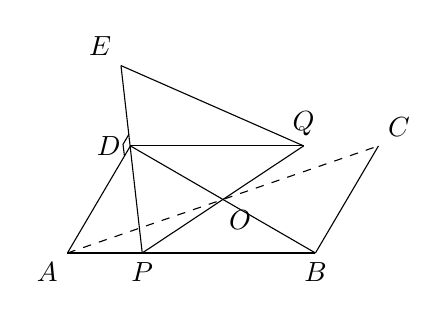
\begin{tikzpicture}
  \coordinate (A) at (0.65,-3.02);
  \coordinate (P) at (1.60,-3.02);
  \coordinate (B) at (3.80,-3.02);
  \coordinate (C) at (4.60,-1.66);
  \coordinate (D) at (1.45,-1.66);
  \coordinate (Q) at (3.65,-1.66);
  \coordinate (E) at (1.33,-0.64);
  \coordinate (O) at (2.58,-2.36);

  % parallelogram sides
  \draw (A) -- (B);
  \draw (B) -- (C);
  \draw (A) -- (D);

  % dashed diagonal AC
  \draw[dashed] (A) -- (C);

  % thin diagonal DB
  \draw (D) -- (B);

  % triangle DEQ-related edges
  \draw (E) -- (P);
  \draw (E) -- (Q);
  \draw (D) -- (Q);
  \draw (P) -- (Q);

  % right angle mark at D
  \draw (1.374,-1.789) -- (1.356,-1.640) -- (1.432,-1.511);

  % labels
  \node[above left] at (E) {$E$};
  \node[left] at (D) {$D$};
  \node[above] at (Q) {$Q$};
  \node[above right] at (C) {$C$};
  \node[below left] at (A) {$A$};
  \node[below] at (P) {$P$};
  \node[below] at (B) {$B$};
  \node[below right] at (O) {$O$};
\end{tikzpicture}
\end{document}
